\documentclass[a4paper,10pt]{report}

\topmargin -2cm
%\topskip0cm
%\footskip0cm
%\headsep0cm
\parindent0cm
\oddsidemargin -1cm
\evensidemargin -1cm
\headheight 2cm
\textheight 24cm
\textwidth 18cm

\author{Daniel W\"aber (4049590)}
\title{\"Ubung}

\usepackage{ucs}
\usepackage[utf8x]{inputenc}
\usepackage{german}
\usepackage{color}
\usepackage{url}
\usepackage{graphicx}
\usepackage{algorithmic}

\pagestyle{empty}
\usepackage{makeidx}
\usepackage{amsmath}
\usepackage{amsfonts}
\usepackage{amssymb,euscript}
\usepackage{dsfont}
\usepackage{listings}
\usepackage{enumerate}
\newfont{\Fr}{eufm10}
\newfont{\Sc}{eusm10}
\newfont{\Bb}{msbm10}
\newcommand{\limin}{\lim_{n\rightarrow\infty}}
\newcommand{\limix}{\lim_{x\rightarrow\infty}}
\newcommand{\limun}{\lim_{n\rightarrow -\infty}}
\newcommand{\limux}{\lim_{n\rightarrow -\infty}}
\newcommand{\limx}{\lim_{x\rightarrow x_0}}
\newcommand{\limh}{\lim_{h\rightarrow 0}}
\newcommand{\defi}{\paragraph{Definition:}}
\newcommand{\bew}{\paragraph{Beweis:}}
\newcommand{\satz}{\paragraph{Satz:}}
\newcommand{\bsp}{\paragraph{Beispiel:}}
\newcommand{\lemma}{\paragraph{Lemma:}}
\newcommand{\N}{\mathds{N}}
\newcommand{\F}{\mathds{F}}
\newcommand{\Z}{\mathds{Z}}
\newcommand{\Q}{\mathds{Q}}
\newcommand{\R}{\mathds{R}}
\newcommand{\G}{\mathds{G}}
\newcommand{\C}{\mathds{C}}
\newcommand{\K}{\mathds{K}}
\newcommand{\A}{\mathds{A}}
\newcommand{\E}{\mathcal{E}}
\renewcommand{\P}{\mathcal{P}}
\newcommand{\sigA}{$\sigma$-Algebra }
\newcommand{\qed}{$\hfill\blacksquare$}
\newcommand{\arsinh}{\operatorname{arsinh} }
\newcommand{\arcosh}{\operatorname{arcosh} }
\newcommand{\gdw}{ $ \Leftrightarrow $ }
\newcommand{\tf}{ $ \Rightarrow $ }
\newcommand{\mgdw}{\Leftrightarrow}
\newcommand{\mtf}{\Rightarrow}
\newcommand{\Bild}{\text{Bild}}
\newcommand{\Kern}{\text{kern}}
\newcommand{\rg}{\text{rg}}
\newcommand{\deff}{\text{deff}}

\newcommand{\alphato}{\underset{\alpha}\to}
\newcommand{\betato}{\underset{\beta}\to}
\newcommand{\etato}{\underset{\eta}\to}
\newcommand{\ito}{\underset{i}\to}
\newcommand{\sto}{\underset{s}\to}
\newcommand{\kto}{\underset{k}\to}
\newcommand{\xto}{\underset{x}\to}

\usepackage{fancyhdr}
\pagestyle{fancy}
\lhead{Daniel Waeber\\Alex Muenn}
\chead{"Ubungsblatt \nr\\\today}
\rhead{Bildverarbeitung}


\newcommand{\nr}{6}
\lstset{language=matlab}

\begin{document}

\section*{Eingangsbild}
\begin{figure}[H]
\begin{center}

\includegraphics[width=60mm]{u07/smalloma.eps}
\end{center}
\end{figure}

\section*{Aufgabe 1 - Bilineare Interpolation}
Lineare Umsetzung der Erkl\"arung aus der Vorlesung:
\begin{enumerate}
\item Benachbarte Pixelwerte betrachten ($a,b,c,d$)
\item Anwendung der bereits umgeformten Gleichungen ($x = \frac{1}{4}(\frac{1}{4}f_1 + \frac{3}{4}f_2)) + \cdots$) 
      wobei je nach Zielpixel das Seitenverh\"altnis variiert
\end{enumerate}

\begin{lstlisting}[language=matlab,caption=Approxiamation der vier neuen Pixel]
R(x2-1,y2-1) = 9*a + 3*b + 3*c + 1*d;
R(x2  ,y2-1) = 3*a + 9*b + 3*c + 1*d;
R(x2  ,y2  ) = 3*a + 3*b + 9*c + 1*d;
R(x2-1,y2  ) = 1*a + 3*b + 3*c + 9*d;
\end{lstlisting}


\begin{figure}[H]
\begin{center}
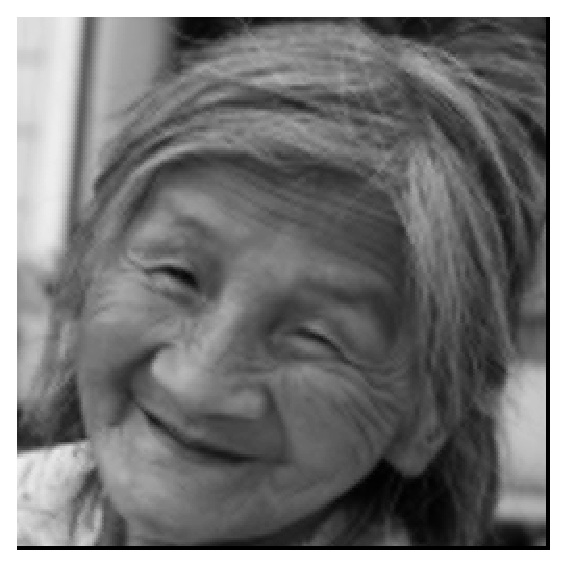
\includegraphics[width=100mm]{u07/task1.eps}
\end{center}
\caption{Ergebnis der bilinearen Interpolation}
\end{figure}

\section*{Aufgabe 2 - Bikubische Interpolation}
Auch hier implementierten wir das in der Vorlesung vorgestellte Verfahren. 
Im Kern geht es darum eine interpolierte Oberfl\"ache zwischen vier Punkten
zu berechnen, die dazwischenliegenden (fehlenden) Informationen am besten 
approximiert.\\
Diese Aufgabe l\"asst sich als lineares Problem $A\alpha=x$ darstellen (siehe VL),
wobei $A$ unsere Interpolationsmatrix ist und $x$ der Eingangsvektor mit seinen vier
Pixelwerten (Nachbarn) und deren Ableitungen in alle Richtungen (12 Werte).\\
$A$ bzw. ihre Inverse um auch $A^{-1}\cdot x = \alpha$ l\"osen zu k\"onnen
sind statische Elemente. In jedem Durchgang wird lediglich:

\begin{enumerate}
\item Nachbarwerte ``holen''
\item Der Eingangsvektor $x$ erstellt
\item Das Gleichungssystem gel\"ost\ldots nach $\alpha$, man erh\"alt die 
      Interpolation zwischen den vier Pixelwerten
\item Berechnen der neuen Farbwerte auf der interpoloierten Ebende durch 
      Einfluss der Seitenverh\"altnisse (Betrachtung des Intervalls $[0,1]$)
\end{enumerate}

\begin{lstlisting}[language=matlab,caption=Eigentliche Berechnung der interolierten Werte]
 u=1/4;
 v=1/4;
 R(x2-1,y2-1) = [u^0*v^0 u^0*v^1 u^0*v^2 u^0*v^3 u^1*v^0 u^1*v^1 u^1*v^2 u^1*v^3 ...
                 u^2*v^0 u^2*v^1 u^2*v^2 u^2*v^3 u^3*v^0 u^3*v^1 u^3*v^2 u^3*v^3 ] * a;
 u=1/4;
 v=3/4;
 R(x2  ,y2-1) = [u^0*v^0 u^0*v^1 u^0*v^2 u^0*v^3 u^1*v^0 u^1*v^1 u^1*v^2 u^1*v^3 ...
                 u^2*v^0 u^2*v^1 u^2*v^2 u^2*v^3 u^3*v^0 u^3*v^1 u^3*v^2 u^3*v^3 ] * a;
 u=3/4;
 v=1/4;
 R(x2-1,y2  ) = [u^0*v^0 u^0*v^1 u^0*v^2 u^0*v^3 u^1*v^0 u^1*v^1 u^1*v^2 u^1*v^3 ...
                 u^2*v^0 u^2*v^1 u^2*v^2 u^2*v^3 u^3*v^0 u^3*v^1 u^3*v^2 u^3*v^3 ] * a;
 u=3/4;
 v=3/4;
 R(x2  ,y2  ) = [u^0*v^0 u^0*v^1 u^0*v^2 u^0*v^3 u^1*v^0 u^1*v^1 u^1*v^2 u^1*v^3... 
                 u^2*v^0 u^2*v^1 u^2*v^2 u^2*v^3 u^3*v^0 u^3*v^1 u^3*v^2 u^3*v^3 ] * a;
\end{lstlisting}

\begin{figure}[H]
\begin{center}
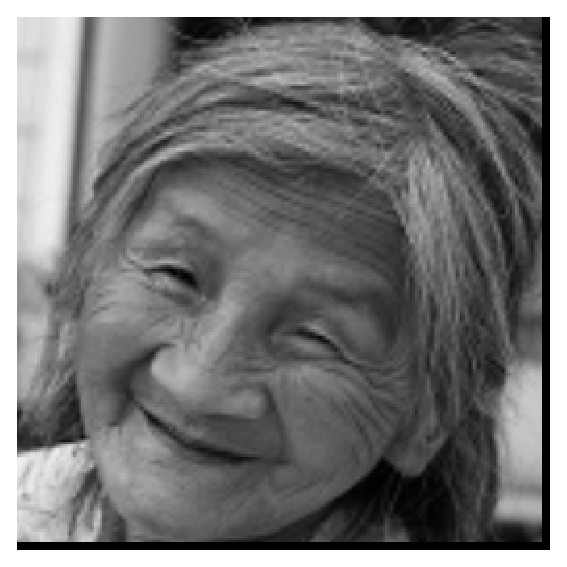
\includegraphics[width=100mm]{u07/task2.eps}
\end{center}
\caption{Ergebnis der bikubischen Interpolation}
\end{figure}

\paragraph{Zusammenfassung/Vergleich}
An den Abbildungen erkennt man unmittelbar einen Unterschied zwischen den beiden 
Interpolationsverfahren. Die bilineare Interpolation hat zwar einen deutlischen
Geschwindigkeitsvorteil, l\"asst aber das Bild eher verschwommen wirken.
Die bikubische Interpolation erzeugt ein klareres Bild mit der Tendenz zum 
Rauschen an einigen Kanten.

\end{document}
